\paragraph{Behavioral Cloning (BC).} \mbox{} \\ 
Behavioral Cloning is one of the first approach used to learn a task from a set of demonstrations. Generally, it is framed as a Supervised Learning problem. Algorithm \ref{alg:bc} defines the classic procedure used to solve the learning task, where, given the dataset $\mathcal{D}^{E}$, a parameterized learner policy $\pi^{L}_{\theta}$, and a loss-function $\mathcal{L}$, the goal is to find the policy's parameter that minimizes the loss-function, or in other terms, $\theta^{*} = \underset{\theta}{argmin} \ \mathbb{E}_{(\boldsymbol{\tau}, \mathbf{c}) \sim \mathcal{D}^{E}} \ [\mathcal{L}((\boldsymbol{\tau}, \mathbf{c}), \ \pi^{L}_{\theta})]$.
In this setting there are at least two questions to answer: 
\begin{enumerate*}[label=\textbf{(\arabic*)}]
    \item choose whether to optimize in trajectory space or action space;
    \item what kind of representation to use for the policy.
\end{enumerate*}
\newline According to \cite{osa2018algorithmic}, BC methods can be categorized as Model-Free and Model-Based. Moreover, further classification can be based on the fact that the policy is optimized either in the \textit{trajectory space} or in the \textit{action space}. 
%Generally speaking, the most used methods are the model-free methods since, in the context of Behavioral Cloning for Robot Task Learning and Control, the basic assumption is the access to the ground truth state and action, so the problem becomes to mimic the demonstrated behavior. While Model-Based becomes of interest when 
\begin{algorithm}
\caption{Abstract Algorithm for Behavioral Cloning}\label{alg:bc}
\begin{algorithmic}
\Require A set of expert demonstrations $\mathcal{D}^{E}$, a parameterized policy $\pi_{\theta}^{L}$
\Ensure The optimal set of policy parameter $\theta^{*}$
\State Optimize $\mathcal{L}$ w.r.t. policy parameter $\theta$ using $\mathcal{D}^{E}$
\end{algorithmic}
\end{algorithm} 

\textbf{Model-Free methods} learn a policy that reproduces the expert's behavior without learning/estimating system dynamics. Since they do not require neither to estimate the system dynamic nor to learn a reward function, they are simple to implement and do not necessary require system  interactions. 

Model-Free methods that derive policy in the trajectory space were very popular in the context of Model-Free BC for trajectory planning, given their ability to explicitly model constraints (e.g. a smooth convergence to the goal state). In this setting well studied methods are the \textit{Dynamic Movement Primitives} (DMPs) \cite{ijspeert2002learning,ijspeert2013dynamical}, which can represent non-linear movements without losing the stability of the behavior.  
Authors in \cite{ijspeert2013dynamical} formulated the Dynamic Movement Primitive for a single DoF point-to-point trajectory using the following set of non-linear differential equations: \begin{equation}
    \tau \dot{y} = \beta_{s}(\alpha_{s}(g-s)- y) + f(z)
\end{equation}
\begin{equation}
    \tau \dot{s} = y
\end{equation}
\begin{equation}
    \tau \dot{z} = -\alpha_{z} z, \ z(t) = z_{0} \ exp(-\frac{\alpha_{z}}{\tau} t)
\end{equation}
 Where $\beta_{s}, \alpha_{s}, \alpha_{z}$ are constants, $s$ is the system state, $z$ is the phase-variable function of time $t$, and $f$ is the forcing-term which describes the trajectory non-linear behavior. Generally, $f$ is a linear combination of basis-function $\psi_{i}(z)$ (e.g., Gaussian basis function), i.e., $f(z(t)) = (g-s_{0}) \sum_{i=1}^{M}\psi_{i}(z(t))\omega_{i}z$. Basically, a DMP describes a point-attractor system, where the current system state $s$ must converge to the goal state $g$, starting from $s_{0}$. In this setting, the aim is to learn the set of weights, $\left\{\omega_{i}, i=1,\dots,M\right\}$, which can be obtained by solving a supervised learning problem with loss function $\mathcal{L}_{DMP} = \sum_{t=0}^{T}(f_{target}(t) - f(z(t)))^{2}$, where $f_{target}(t) = \tau^{2} \ \ddot{s}^{E} - \beta_{s}(\alpha_{s}(g - s^{E})-\tau \dot{s}^{E})$. DMPs formulation has been used in the context of robotic manipulation. For example in \cite{meier2011movement_primitive,caccavale2019kinesthetic,agostini2020manipulation} the problem of task decomposition was faced, and DMPs have been used to model the sub-tasks. However, DMPs formulation has a series of problems related to: \begin{enumerate*}[label=(\textbf{\alph*})]
    \item how to handle stochasticity in demonstration;
    \item how to explicitly define basis function, given the desired behavior;
    \item how to handle arbitrary desired trajectories, with intermediate via-points;
    \item how to handle complex high-dimensional inputs. 
\end{enumerate*}
For all the above mentioned problems some solutions have been proposed. For example, the stochasticity problem was addressed in \cite{paraschos2013ProMPs}, where the Probabilistic Movement Primitives (ProMPs) method was proposed. In ProMPs the probability of observing a trajectory $\boldsymbol{\tau}$ is written as $\boldsymbol{\tau} = \underset{t}{\prod} \ \mathcal{N}(s(t)|\Psi(z(t))^{T}\omega, \Sigma_{s})$, where $\Psi$ is a time-dependent basis matrix. As in DPMs, the goal is to find the weights $\omega$, by solving a supervised learning problem. As for the second problem, other trajectory representations have been proposed based on Hidden Markov Model, Gaussian Mixture Models, Kernelized Movement Primitives. However, all these alternatives scale bad when the goal is to learn a policy starting from visual observations. To handle such complex high-dimensional input Deep Architecture have been proposed, which will be explained in detail in the next sections. 
%As for the second problem, the idea proposed in the literature is to use deep architecture to learn the DMPs parameters \cite{ridge2020training_nn_dmps}. 
\newline Regarding the methods that derive the policy in the action-space. One of the primal work was \cite{pomerleau1988alvinn}, which proposed \textit{ALVINN}, an autonomous vehicle driving system based on a Neural Network, that infers the steering angle, given a synthetic camera image as input. The network was trained on pairs (image, steering-angle) and the training procedure was defined as a supervised classification problem, since the steering-angle was discretized over 45 units. This work immediately emphasized the problem of compounding-error, caused by covariate-shift phenomena. This issue occurs because an action $a_{t}$ influences the next state $s_{t+1}$, which represents the next sample, violating the i.i.d assumption of Supervised Learning and generating a test-data distribution, that may be different from the training one. This phenomena has a relevant consequence on the expected performance of the system. Indeed, assuming to have a system that makes an error with probability $\epsilon$, and a task with time-horizon $T$, then, due to compounding error, a supervised learner reaches a total cost of $O(\epsilon \ T^{2})$, rather than $O(\epsilon \ T)$ \cite{ross2010efficient_reductions,ross2011dagger}. To attenuate this problem, interactive supervised learning algorithms have been proposed, such as the well-known \textit{DAgger} \cite{ross2011dagger}. Algorithm \ref{alg:dagger} describes the DAgger procedure. It is an aggregation strategy, based on the idea to train the policy $\pi^{L}$ under the state-distribution induced by the policy itself, but with the correct action performed by the expert. The main problem with DAgger is that it requires the expert to interact with the system during the training, introducing both safety and data-efficiency problems, especially when the system does not provide the human expert with sufficient control authority during the sampling process \cite{laskey2017comparing_hc_rc}. \begin{algorithm}
\caption{DAgger Algorithm \cite{ross2011dagger}}\label{alg:dagger}
\begin{algorithmic}
\Require Initial Dataset $D \leftarrow \emptyset$, Initial policy $\pi^{L}_{1}$
\Ensure The best policy $\pi^{L}_{i}$
\For {$i=1, \dots N$}
    \State Sample $T-step$ trajectories using $\pi^{L}_{i}$
    \State Let $D_{i} = {(s_{t}, \pi^{E}(s_{t}))}$, state $s_{t}$ visited by policy $\pi^{L}_{i}$, 
    \State and actions given by the expert
    \State Aggregate Dataset, $D \leftarrow D \bigcup D_{i}$
    \State Train policy $\pi^{L}_{i}$ on $D$
    \State Let $\pi^{L}_{i+1} = \beta_{i}\pi^{E} + (1- \beta_{i})\pi^{L}_{i}$
\EndFor
\end{algorithmic}
\end{algorithm}
\newline Human-Guided DAgger (HG-DAgger) \cite{kelly2019hg_dagger} is an extension of the classic DAgger strategy, in which the human expert observes the rollout of the current policy, so if the agent has entered an unsafe region of the state space, the expert takes control and guides the system to a safe and stable region. In \cite{jang2022bc_z} was shown how HG-DAgger can be effectively used in the context of robotic manipulation. Indeed, starting from the same total number of episodes, a policy trained with only expert demonstration has a significantly lower success rate than a policy trained on a dataset with both expert demonstrations and expert adjustments. In the context of Interactive Learning for Robot Manipulation, other works of interest include \cite{mandlekar2020human_in_the_loop,chisari2022correct}. In \cite{chisari2022correct}, a human expert provides both corrective and evaluative feedback. %(Figure \ref{fig:feedback}).
The former consists in the human that takes control of the robot to adjust the trajectory, the latter consists in a scalar weight $q$, set to 1 if the trajectory is satisfactory, 0 the trajectory is not satisfactory, $\alpha$ if the trajectory is adjusted by the expert, where $\alpha$ is the ratio between non-corrected and corrected samples. Then a Neural Network % in Figure \ref{fig:architecture}
was trained by minimizing a weighted version of the maximum-likelihood $\mathcal{L}(a_{t},s_{t}) = - q \ log(\pi^{L}_{\theta}(a_{t}|s_{t}))$. Real-world experiments show that with a training time of \textbf{41 minutes}, including environmental reset, it was possible to have an agent capable of performing tasks such as picking up a cube or pulling a plug.
%\begin{figure}[htbp]
    \begin{subfigure}{0.45\textwidth}
         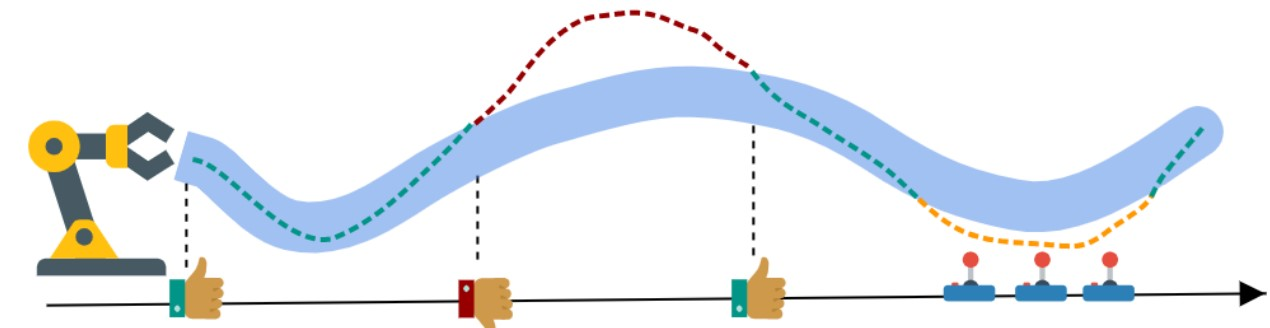
\includegraphics[width=\textwidth]{Figures/images/correct-me-if-i-am-wrong/feedback.jpg}
         \caption{Evaluative feedback: the expert labels the sub-trajectory as satisfactory or not. Corrective feedback: the human guides the robot towards the correct trajectory}
         \label{fig:feedback}
    \end{subfigure}
    \hfill
    \begin{subfigure}{0.50\textwidth}
         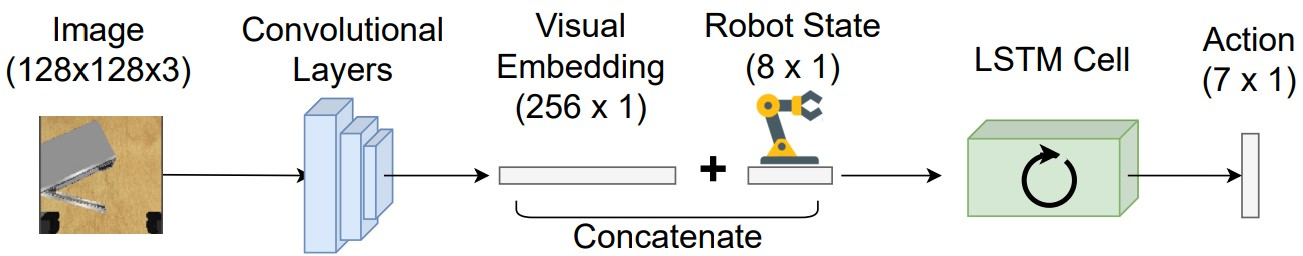
\includegraphics[width=\textwidth]{Figures/images/correct-me-if-i-am-wrong/correct_me_architecture.jpg}
         \caption{Policy architecture: The input is an RGB image of the scene, the output is the desired end-effector pose and the gripper state}
         \vspace{0.5cm}
         \label{fig:architecture}
    \end{subfigure}
    \caption{(\ref{fig:feedback}) Representation of the meaning of the feedback, (\ref{fig:architecture}) Policy architecture proposed in \cite{chisari2022correct}}
    \label{fig:correct_me_if_im_wrong}
\end{figure}

%Classic Behavioral Cloning

Despite the covariate-shift problem, \cite{zhang2018deep_vr_teleoperation} showed that very interesting performance can be obtained in the context of Robot Manipulation Task, by means of Behavioral Cloning and high quality demonstrations given by teleportation system. In this work, a CNN was trained to predict the desired linear-velocity and angular-velocity of the end-effector (Figure \ref{fig:deep_bc}), with the binary gripper state (open/close), given in input the current RGB-D observation of the scene, and the position of three points of the end-effector, during the last 5 time-steps. The system was tested on 10 tasks, and the performance are reported in Table \ref{table:deep_vr_teleoperation_results}. The proposed system achieved a high success rate while evaluating all the tasks. The tests were carried out from different initial conditions but still quite similar to those present in the training set (e.g., the initial object positions have been uniformly distributed within the training regime, with random local variations around these positions). The analysis of failure cases showed that the leading cause of errors was the inability to detect critical points in the task execution, such as closing/opening the gripper to pick/place the object or detect the position of the object of interest in order to avoid collision with it.\begin{figure}[bt]
    \centering
    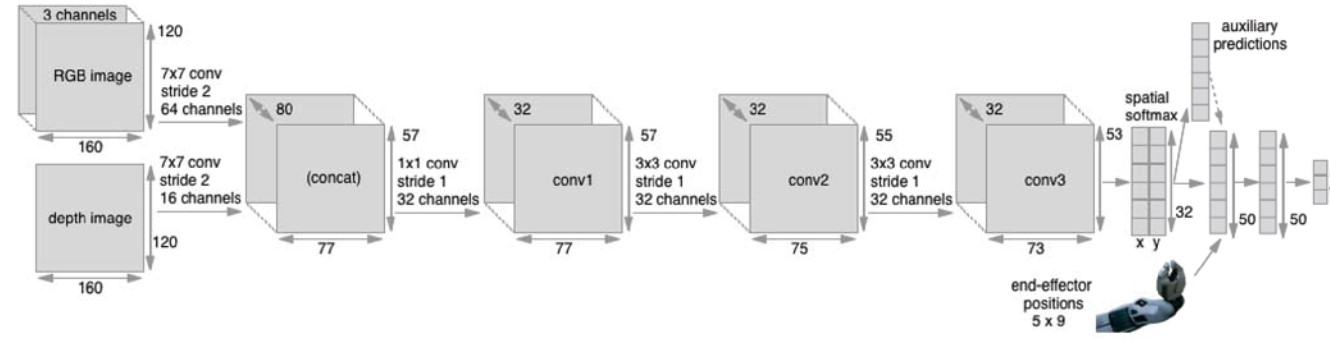
\includegraphics[width=0.8\textwidth]{Figures/images/deep_imitation_bc/deep_imitation_bc.jpg}
    \caption{Architecture proposed in \cite{zhang2018deep_vr_teleoperation}}
    \label{fig:deep_bc}
\end{figure}
\begin{table}
\centering
\caption{Statistics of Training set, and Test Success rate \cite{zhang2018deep_vr_teleoperation}}
\label{table:deep_vr_teleoperation_results}
\resizebox{\linewidth}{!}{%
\begin{tabular}{c|c|c|c|c|c|c|c|c|c|c}
task                                                                                                                                   & reaching & grasping & pushing & plane & cube & nail & grasp-and-place & grasp-drop-push & grasp-place-x2 & cloth  \\ 
\hline
\rowcolor[rgb]{0.753,0.753,0.753} \#demo                                                                                               & 200      & 180      & 175     & 319   & 206  & 215  & 109             & 100             & 60             & 100    \\ 
\hline
\begin{tabular}[c]{@{}c@{}}demo duration \\(min)\end{tabular}                                                                          & 13.7     & 11.1     & 16.9    & 25.0  & 12.7 & 13.6 & 12.3            & 14.5            & 11.6           & 10.1   \\ 
\hline
\rowcolor[rgb]{0.753,0.753,0.753} \begin{tabular}[c]{@{}>{\cellcolor[rgb]{0.753,0.753,0.753}}c@{}}Test success rate\\(\%)\end{tabular} & 91.6     & 97.2     & 98.9    & 87.5  & 85.7 & 87.5 & 96.0            & 83.3            & 80.0           & 97.4  
\end{tabular}
}
\end{table}\unskip Another important aspect to note is that, for each task, the network was trained from scratch. This is not a desired property for a highly adaptable system, as stated in Section \ref{sec:intro}. For this reason, methods based on Meta-Learning algorithms have been proposed. The idea behind Meta-Learning is to train a model on a variety of tasks, in such a way that it can solve a new tasks, using only a small number of training samples \cite{finn2017maml}. Algorithm \ref{alg:maml} describes the steps followed by the \textit{Model-Agnostic Meta-Learning} (MAML) algorithm \cite{finn2017maml}, that is the base for different methods which apply One-shot Imitation Learning in the context of Behavioral Cloning \cite{finn2017one_shot_visual_il,yu2018daml,yu2018one_shot_hil}.\begin{algorithm}[h]
\caption{Model-Agnostic Meta-Learning (MAML) \cite{finn2017maml}}
\label{alg:maml}
\begin{algorithmic}
\Require Distribution over tasks $p(\mathcal{T})$
\State Randomly initialize $\theta$
\While {$i=1, \dots N$}
    \State Sample batch of tasks $ \mathcal{T}_{i} \sim p(\mathcal{T})$
    \For {\textbf{all} $\mathcal{T}_{i}$}
        \State Evaluate $\nabla_\theta \mathcal{L}_{\mathcal{T}_{i}}(f_{\theta})$ w.r.t. $K$ examples
        \State Compute adapted parameters with gradient descent: $\theta'_{i} = \theta - \alpha \nabla_\theta\mathcal{L}_{\mathcal{T}_{i}}(f_{\theta})$
    \EndFor
    \State Update $\theta \leftarrow \theta - \beta \nabla_\theta \sum_{\mathcal{T}_{i} \sim p(\mathcal{T})} \mathcal{L}_{\mathcal{T}_{i}}(f_{\theta'_{i}})$
\EndWhile
\end{algorithmic}
\end{algorithm}
\newline In \cite{finn2017one_shot_visual_il}, MAML algorithm was used to prove the effectiveness of Meta-Learning in the context of real robot manipulation, with visual observations, as opposite to \cite{duan2017one_shot_il}. A Convolutional Neural Network was trained by following the Algorithm \ref{alg:maml}, using as loss-function the Mean Squared Error, computed between the predicted action and the ground truth one. For real-robot experiments a dataset of \textbf{1300} placing demonstrations (i.e., place an holded object in a target container), containing near to \textbf{100} different objects, was collected through teleportation. The trained system was tested by performing the adaptation step on one video demonstration, over 29 new objects, moreover, between the video demonstration and the actual execution, the objects configuration was changed. In this setting the system reached the $\mathbf{90\%}$ of success rate, outperforming baseline methods based on LSTM \cite{duan2017one_shot_il}, and contextual network (i.e., a CNN that takes in input the current observation and the image representing the target state). 
In \cite{yu2018daml}, the \textit{Domain Adaptive Meta-Learning} algorithm (DAML) was proposed with the goal of learning to infer a policy from a single human demonstration. To achieve it, a two-step algorithm was proposed. In the first-step, called \textbf{Meta-Learning step}, given in input, for each task $\mathcal{T}$, a set of human demo $\mathcal{D}^{h}_{\mathcal{T}}$ and a set or robot demo $\mathcal{D}^{r}_{\mathcal{T}}$ (Figure \ref{fig:daml}), the \textit{initial policy parameters} $\theta$ and the \textit{adaptive loss} parameters $\psi$ are learned, solving the problem in Formula \ref{eq:daml}. \begin{equation}
 \label{eq:daml}
 \underset{\theta,\psi}{\min} \sum_{\mathcal{T} \sim p(\mathcal{T})} \sum_{\mathbf{d}^{h} \sim D^{h}_{\mathcal{T}}} \sum_{\mathbf{d}{^r} \sim D^{r}_{\mathcal{T}}} \mathcal{L}_{BC}(\theta - \alpha \nabla_\theta\mathcal{L}_{\psi}(\theta,\mathbf{d}^{h}), \mathbf{d}^{r})
\end{equation}

\newline Where the outer loss is $\mathcal{L}_{BC}(\phi,\mathbf{d^{r}}) = \sum_{t} log(\pi_{\phi}(a_{t}|s_{t},o_{t}))$, and the inner-loss $\mathcal{L}_{\psi}$, is the learned adaptive loss, which is used during the \textbf{Meta-Test step}, where the policy parameters are adapted with gradient descent given in input a video of human demo of a new task $\mathcal{T}$, i.e., $\phi_{\mathcal{T}} = \theta - \alpha \nabla_{\theta} \mathcal{L}_{\psi}(\theta, \mathbf{d^{r}})$. Experimental evaluation on tasks such as placing, pushing, and pick-and-place, has shown that: \begin{enumerate*}[label=\textbf{(\alph*)}]
    \item the system was able to generalize across both new objects and objects configuration starting from only a single human-demonstration;
    \item a performance degradation was observed in large domain-shift experiments, such as novel backgrounds and different camera view-points.
\end{enumerate*}\begin{figure}[htbp]
    \centering
    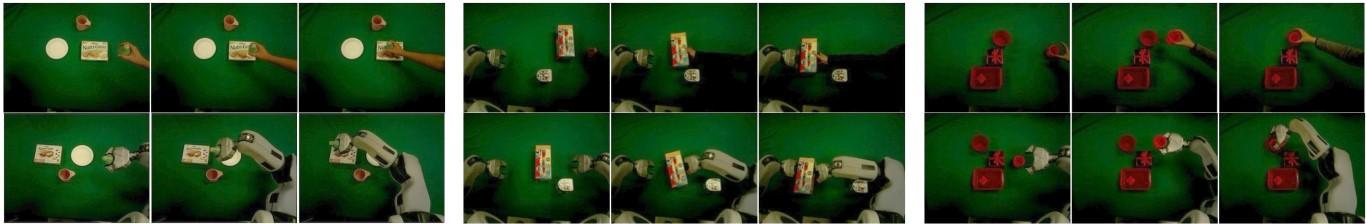
\includegraphics[width=\textwidth]{Figures/images/daml/tasks.jpg}
    \caption{Tasks performed in \cite{yu2018daml}. (Top row) Human demonstration, (Bottom row) robot demonstration. (Left) Placing task, (Middle) pushing task, (Right) pick-and-place task.}
    \label{fig:daml}
\end{figure}


All the works described up to now, consider the task distribution $p(\mathcal{T})$ as composed of one-single task, but with many different variations \cite{finn2017one_shot_visual_il} or different, but related tasks \cite{yu2018daml}. Very recent methods try to generalize BC to a huge variety of tasks \cite{jang2022bc_z,mandi2022towards_more_generalizable_one_shot}.
In \cite{jang2022bc_z}, a large-scale dataset containing \textbf{100} diverse manipulation tasks was collected. The demonstrations were collected through both expert teleoperation and shared autonomy process (HG-DAgger \cite{kelly2019hg_dagger}). The demonstrated tasks were related to pick-and-place, grasp, pick-and-drag, pick-and-wipe, and push skills. The dataset was used to train the network in Figure \ref{fig:bcz_architecture}. As it can be noted the samples were composed by current robot observation, and a conditioning represented by either a natural language description or a video demo. The idea was that training a conditioned policy over the current observation $o_{t}$, and a task representation $c_{t}$, $\pi^{L}(a_{t}|o_{t}, c_{t})$, it would allow the policy to generalize over new tasks in a zero-shot manner (i.e., without any fine-tuning). Experimental results shown that, over 28 held-out tasks, containing both completely new objects, and known objects but in different tasks, an average success rate of \textbf{38\%} was reached in the easiest setting, with only one distractor and with natural language instruction. The success rate dropped to \textbf{4\%} in the hardest setting with 4 distractors and video conditioning. %These bad performance can be justified by the classic training procedure followed, while different advantages may be gained from Meta-Learning algorithms, and by how the human video embedding was obtained, through a CNN on a 4x5 matrix of images, with a completely loss of temporal information.
In their analysis, the authors pointed out that the system did not fail to identify the object, but in what they called ``\textbf{last-centimeter errors}", i.e., failing to close the gripper, failing to let go of objects, or a near miss of the target object when letting go of an object in the gripper. 
\begin{figure}[htb!]
    \centering
    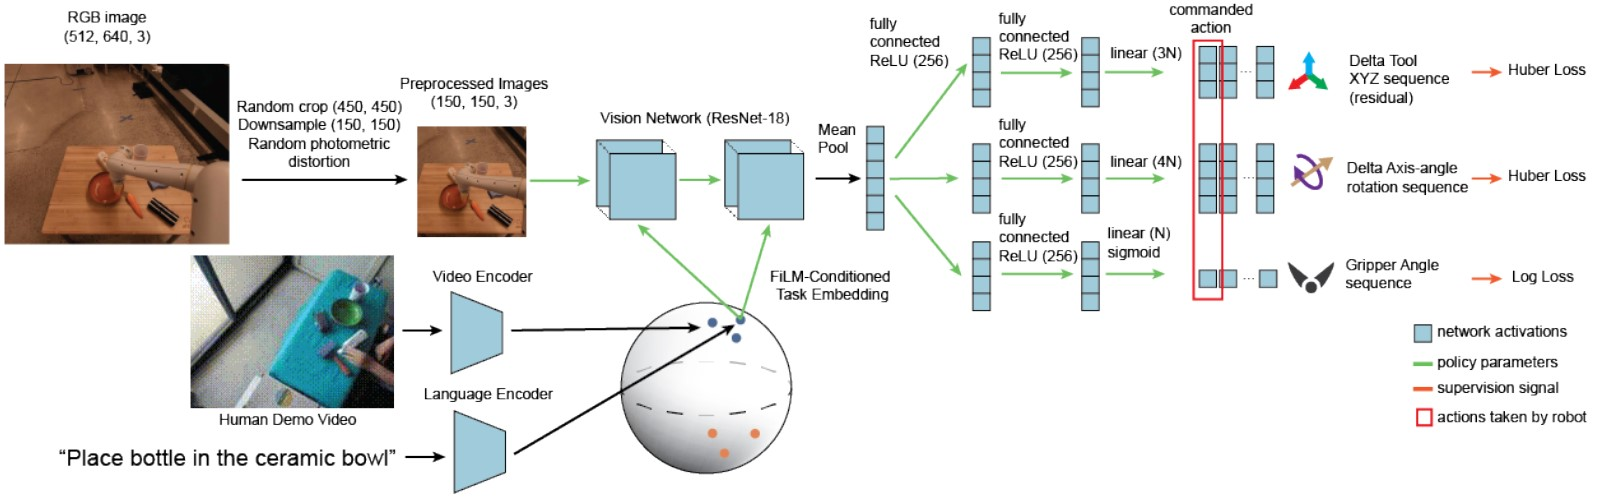
\includegraphics[width=0.9\textwidth]{Figures/images/bc_z/bc-z-network.jpg}
    \caption{Architecture proposed in \cite{jang2022bc_z}}
    \label{fig:bcz_architecture}
\end{figure}
Authors in \cite{mandi2022towards_more_generalizable_one_shot} did a further step towards Multi-task Imitation Learning. They proposed Multi-task One-Shot imitation with self-AttentIon and Contrastive Learning (MOSAIC), an architecture designed to solve the multi-task imitation learning problem by incorporating two key components: \begin{enumerate*}[label=\textbf{(\arabic*)}]
    \item a time-contrastive loss as additional supervision for representation learning, with the aim to obtain similar embeddings for temporally close-by frames;
    \item a self-attention model architecture with the aim to extract contextual information from demonstrations, used by the Neural Network to infers the action.
\end{enumerate*} The system was tested on 7 different tasks, with a set of 61 variations, and compared against other one-shot imitation learning methods \cite{yu2018daml,dasari2021transformers_one_shot}. The results in Table \ref{table:mosaic} show that MOSAIC outperforms previous methods in the Single-Task One-shot Imitation Learning Setting, i.e., one-task with multiple variations and tested on an unseen variations. Moreover, when tested in a Multi-Task setting, i.e., holding-out the task to test and training on the remaining 6 tasks, the method is not able to wholly generalize to the novel unseen task starting from a single demonstration, while, the sucess rate increases if the network is fine-tuned on the hold-out task, as expected. The results reported by the different methods pointed out how there is a wide room for improvement in the context of both Single-Task and Multi-Task Few-shot Imitation Learning methods, which are particularly promising when it comes to task-level generalization, because the intent of the new task is correctly captured, especially in the case of conditioned policies. However, the success rate in task execution is relatively low for several reasons that can range from difficulty in identifying key points in task execution (e.g., the robot has approached the object and, therefore, the gripper must be closed) to compounding error, which leads to new observations different from those in the training set (e.g., the robot did not grasp the object correctly). As a result, the robot cannot complete the task because it performs actions inconsistent with the state of the task itself. Possible improvements can range from using a multi-modal system based on video and tactile information in order to make explicit the transition between consecutive task phases, to adding bad demonstrations combined with recovery behavior during data collection. 
%\begin{figure}[htb]
    \centering
    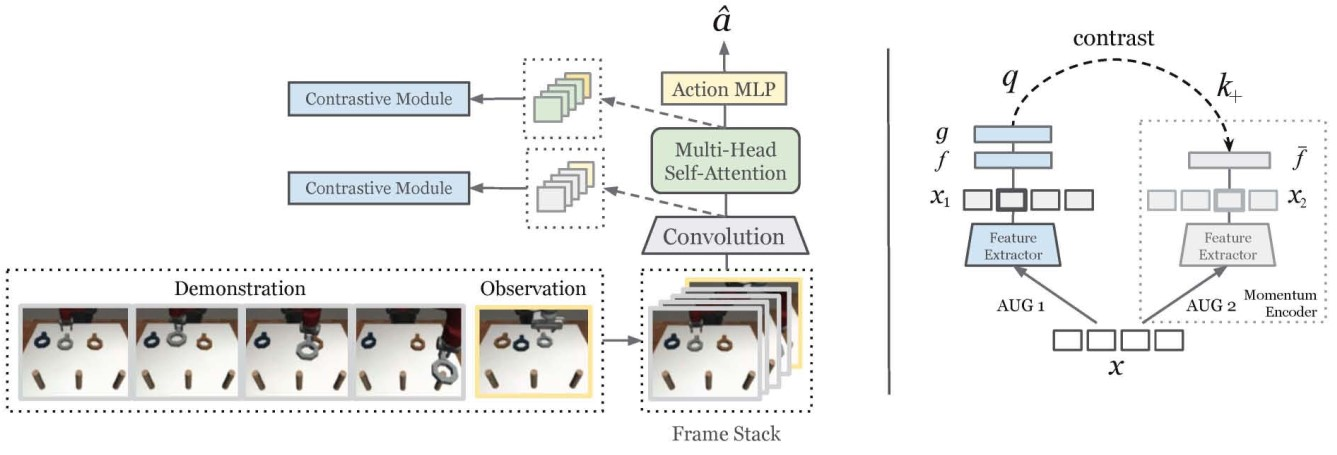
\includegraphics[width=0.9\textwidth]{Figures/images/mosaic/mosaic.jpg}
    \caption{MOSAIC architecture \cite{mandi2022towards_more_generalizable_one_shot}}
    \label{fig:mosaic}
\end{figure}

\begin{figure}[htb]
    \centering
    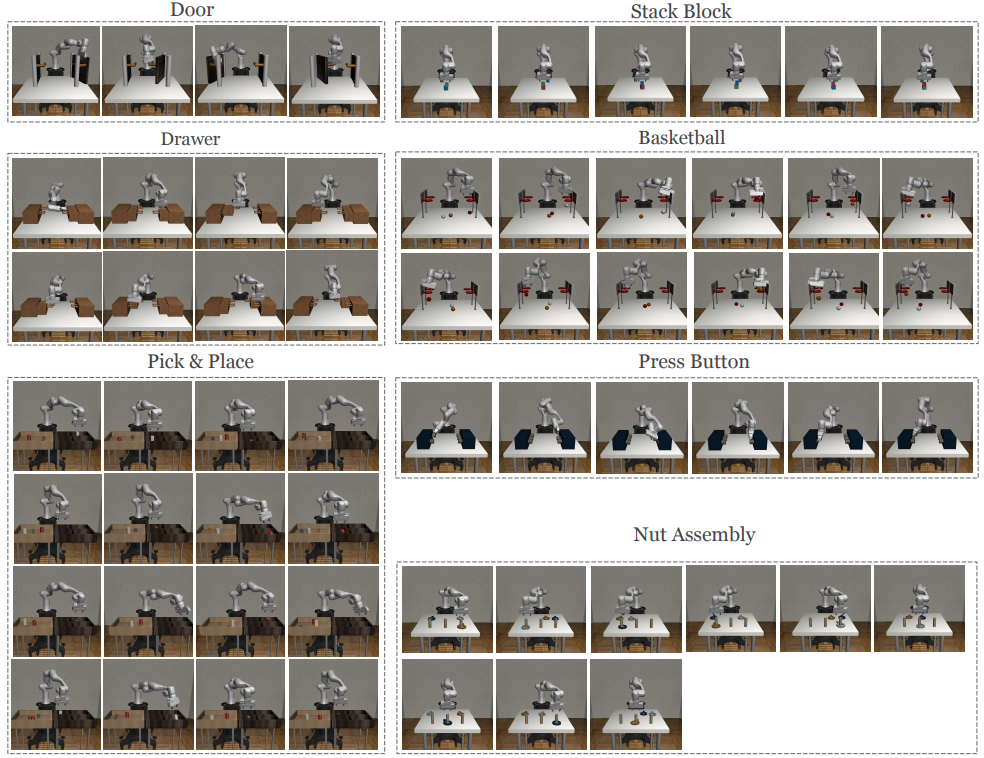
\includegraphics[width=0.9\textwidth]{Figures/images/mosaic/mosaic_tasks.png}
    \caption{MOSAIC \cite{mandi2022towards_more_generalizable_one_shot} proposed tasks}
    \label{fig:mosaic_tasks}
\end{figure} 
\begin{table}
    \centering
    \small\caption{Results obtained in single-task and multi-task one-shot imitation learning \cite{mandi2022towards_more_generalizable_one_shot}.}
    \label{table:mosaic}
    \resizebox{\linewidth}{!}{%
    \begin{tabular}{>{\centering\hspace{0pt}}m{0.187\linewidth}>{\centering\hspace{0pt}}m{0.081\linewidth}>{\centering\hspace{0pt}}m{0.223\linewidth}>{\centering\hspace{0pt}}m{0.223\linewidth}>{\centering\arraybackslash\hspace{0pt}}m{0.223\linewidth}} 
    \toprule
    Task                                        & Setup  & DAML \cite{yu2018daml}          & T-OSIL \cite{dasari2021transformers_one_shot}        & MOSAIC \cite{mandi2022towards_more_generalizable_one_shot}         \\ 
    \hline
    \multirow{2}{*}{\Centering{}Open door}      & single & 23.3~$\pm$ 5.2 & 57.9~$\pm$~7.1 & \textbf{67.1} $\pm$ \textbf{5.5}   \\
                                                & multi  & 10.8~$\pm$ 5.4 & 49.2~$\pm$ 6.0 & \textbf{68.3}~$\pm$~\textbf{6.3}  \\ 
    \hline
    \multirow{2}{*}{\Centering{}Open drawer}    & single & 15.4~$\pm$ 5.5 & 57.5~$\pm$~3.9 & \textbf{65.4}~$\pm$~\textbf{3.4}  \\
                                                & multi  & 3.3~$\pm$~1.4  & 53.3~$\pm$~4.0 & \textbf{55.8}~$\pm$~\textbf{3.6}  \\ 
    \hline
    \multirow{2}{*}{\Centering{}Press button}   & single & 62.8~$\pm$~3.9 & 56.4~$\pm$ 2.4 & \textbf{71.7}~$\pm$ \textbf{3.9}  \\
                                                & multi  & 1.7~$\pm$~0.7  & 63.3 $\pm$ 3.5 & \textbf{69.4}~$\pm$~\textbf{3.4}  \\ 
    \hline
    \multirow{2}{*}{\Centering{}Pick-and-Place} & single & 0.0~$\pm$~0.0  & 74.4~$\pm$~2.1 & \textbf{88.5}~$\pm$~\textbf{1.1}  \\
                                                & multi  & 0.0~$\pm$~0.0  & 19.5~$\pm$~0.4 & \textbf{42.1}~$\pm$ \textbf{2.3}  \\ 
    \hline
    \multirow{2}{*}{\Centering{}Stack block}    & single & 10.0~$\pm$~1.8 & 13.3~$\pm$~2.6 & \textbf{79.3}~$\pm$~\textbf{1.8}  \\
                                                & multi  & 0.0~$\pm$~0.0  & 34.4~$\pm$~3.4 & \textbf{70.6}~$\pm$~\textbf{2.4}  \\ 
    \hline
    \multirow{2}{*}{\Centering{}Basketball}     & single & 0.4~$\pm$~0.3  & 12.5~$\pm$~1.6 & \textbf{67.5}~$\pm$~\textbf{2.7}  \\
                                                & multi  & 0.0~$\pm$~0.0  & 6.9~$\pm$~1.3  & \textbf{49.7}~$\pm$~\textbf{2.2}  \\ 
    \hline
    \multirow{2}{*}{\Centering{}Nut assembly}   & single & 2.2$\pm$~1.4   & 6.3 $\pm$~1.9  & \textbf{55.2}~$\pm$~\textbf{2.8}  \\
                                                & multi  & 0.0~$\pm$~0.0  & 6.3 $\pm$~1.3  & \textbf{30.7}~$\pm$~\textbf{2.5}  \\
    \bottomrule
    \end{tabular}
    }
    \end{table}
\newline The methods presented up to now partially solve the problems related to compounding error and task-generalization. Another relevant problem related to Behavioral Cloning, and more in general to Learning from Demonstration, is the execution of \textbf{multi-stage long-horizon tasks}. Indeed, it is pretty intuitive to think that a manipulation task is characterized by a modular structure which can be exploited to improve performance, following the idea that each sub-task can be learned more efficiently because each skill is shorter-horizon. In this setting, the main question to answer is: \textit{How can a task be decomposed into the corresponding component skills?} In its classical formulation, this problem can be framed as a classification problem. In a preliminary work \cite{meier2011movement_primitive}, the authors used a set of predefined primitive motions modeled as DMPs. The goal was to recognize these primitives within the demonstrated trajectory using an Expectation-Maximization algorithm. Also, recent methods \cite{caccavale2019kinesthetic,agostini2020manipulation} exploit the DMPs formulation. However, they are not part of the process of task segmentation. For example, in \cite{caccavale2019kinesthetic}, the action segmentation is performed based on either object proximity or explicit human command. When the robot manager identifies a new action, the corresponding DMP is learned, and the sequence of tasks is organized in a hierarchical structure. The problem of task-segmentation was also solved starting from an unconstrained video demonstrations labeled with commands \cite{xu2018neural_task_programming}, activity \cite{yang2015robot}, or completely unlabeled \cite{yu2018one_shot_hil,Mandlekar2020GTI}. In \cite{yu2018one_shot_hil}, the authors proposed an extension of DAML for multi-stage tasks. The main idea of this work was based on modeling the distribution of tasks as a set of primitives (e.g., reach primitive). During the meta-training phase, two systems were obtained: \begin{enumerate*}[label=(\textbf{\arabic*})]
    \item a human/robot-phase predictor, whose responsibility was to indicate the completion rate of the current primitive given a human video demonstration and a robot video demonstration, respectively;
    \item a Convolutional Neural Network trained according to DAML, which acted as a motion-primitive meta-model policy, parameterized by meta-parameters $\theta$.
\end{enumerate*} During the meta-test phase, given as input a video of human performing a compound task, three steps were defined: \begin{enumerate*}[label=(\textbf{\arabic*})]
    \item extrapolate the set of primitives by using the human-phase predictors;
    \item for each primitive, starting from the meta-parameters $\theta$, find the parameters $\phi_{i}$ by performing gradient descent on the learned loss function $\mathcal{L}_{\psi}$;
    \item execute the policy parameterized by $\phi_{i}$, until the current sub-task is completed (completion detected by the robot-phase predictor).
\end{enumerate*} The work proposed in \cite{Mandlekar2020GTI} addressed the multi-stage long-horizon tasks with a different approach. The authors did not focus on an explicit concept of task segmentation. Indeed, they started with the idea that similar tasks intersect at common regions of the state-space, and proposed a two-stage IL architecture able to exploit this intersecting structure to generalize to unseen start-goal state combinations. These methods are interesting because they allow the execution of a compound task from simple unlabeled videos, thus with as little effort as possible in dataset generation. However, since they do not have semantic information about which part of the task is being executed, they may err on the side of interpretability of actions, which is not the case with methods based on labeled videos or hierarchical structures.

\textbf{Model-Based methods} are characterized by the fact that during the learning process the system dynamic model is learned. There are several reasons why it may be necessary to use the dynamic system model in the context of Learning from Demonstration, for example \begin{enumerate*}[label=\textbf{(\alph*)}]
    \item a difference in the embodiment between the demonstrator and the learner;
    \item a difference in the task execution conditions and parameters.
\end{enumerate*}
Among these methods, the most important aspect is related to how the dynamic model is retrieved, e.g., Gaussian Mixture Model \cite{grimes2009learning_actions_through_imitation} or Gaussian Process \cite{englert2013probabilistic,deisenroth2014multi_task}. In recent years, a significant amount of attention has been placed on systems that can replicate a task from the human video performing a task without any access to ground-truth action. While in the survey mentioned before, these methods were still considered Model-Based Behavioral Cloning. In the current literature, given the increasing amount of works, they can now belong to a new category called Learning from Observation. Methods belonging to this category will be explained in the specific paragraph.  